%\documentclass[11pt]{article}


    

    
    

    
    \hypertarget{network-analysis-an-introduction}{%
\section{1 Network Analysis: An
Introduction}\label{network-analysis-an-introduction}}

    \hypertarget{what-is-network-analysis}{%
\subsection{1.1 What Is Network
Analysis?}\label{what-is-network-analysis}}

Network analysis concerns the study of relationships, often complex
relationships. It can, among other things, assist in understanding
structures (e.g., connections between individuals, organizations,
documents, or viruses), identifying key players in the network (e.g.,
popular individuals, brokers that can connect entities), or examining
spread (e.g., of information, diseases). Applications of network
analysis can be found in a variety of academic disciplines, including
natural sciences, medical science, social sciences, humanities, and law.
In molecular chemistry, network analysis can be used to examine atoms
and how they can be connected through certain chemical bonds. In the
medical field, network analysis can be used to track infections. And in
social science research, one can map communication of a group of social
media users (Figure 1). By mapping who communicates with whom, clusters
may emerge of groups of users who more frequently communicate with
entities within their cluster than with users outside of their cluster.
It can also become apparent who is more central (popular) within the
various clusters or in the network as a whole. Furthermore, one may
identify so-called `brokers', individuals who connect clusters of users
and consequently form the glue that holds the network together.

Figure 1: Example of social media network

(Source: Wikipedia)

Network analysis concerns the measurement and mapping of relationships
between entities. Entities can consist of individuals, groups of
persons, court decisions, molecules, or any other subject or object.
Network analysis relies on the assumption that the structural
relationships between entities (e.g., persons) provide relevant
information that the attributes of those entities alone cannot offer.
The extent to which users are communicative, possess electronic devices,
or are member of social platforms does not provide any or sufficient
insight into how the users relate to one another. Network analysis
reveals those relationships between entities, hence generating relevant
information that the features such as communication skills or platform
membership alone do not offer.

    Below, we will start focusing on what network analysis can mean in a
legal context and how it can be applied to such a context. Before we
discuss this, we very briefly discuss the origins of network analysis.

    \hypertarget{origins-of-network-analysis}{%
\subsection{1.2 Origins of Network
Analysis}\label{origins-of-network-analysis}}

Network analysis stems from graph theory, for which the foundations were
laid by Leonhard Euler in 1736. Euler proved that the problem of `The
Seven Bridges of Königsberg' (currently Kaliningrad, Russia) could not
be solved.

(Source: Google Maps)

Königsberg was divided by the Pregel River, and it had two islands that
were connected to each other and to the city's mainland by seven
bridges. The mathematical problem that Euler solved was to design a walk
that would include the two parts of the mainland as well as the two
islands where the person would cross each of the bridges exactly once.

\begin{figure}
\centering
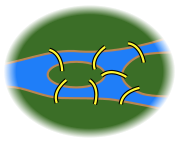
\includegraphics{images/ch1/konisberg_bridges_2.png}
\caption{image2}
\end{figure}

\begin{figure}
\centering
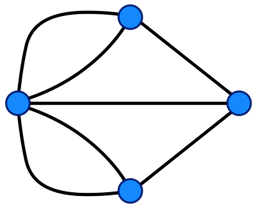
\includegraphics{images/ch1/konisberg_bridges_3.png}
\caption{image2}
\end{figure}

Source: Wikipedia

    Euler demonstrated that the `Seven Bridges of Königsberg' problem does
not have a solution. The possibility of having a walk through town while
crossing every bridge exactly once, depends on the number areas
(mainland + islands) and on the number of bridges. Euler proved that the
desired walk (now knwon as an ``Eulerian path'') could only take place
if the areas are connected and include exactly zero or two areas with an
odd number of bridges. Königsberg had four areas and seven bridges at
the time. Three areas had three bridges and one area had five bridges.
As a result, Euler's rule was violated, as there were four areas with an
odd number of bridges.

The seven bridges were bombed in World War II. Five bridges were
rebuilt. A Eulerian path through the bridges became possible after the
reconstruction (in the figure below:
1-\textgreater2-\textgreater3-\textgreater4-\textgreater5). Now, two
areas (in the figure below: B+C) have two bridges, whereas the other two
areas (in the figure below: A+D) have three bridges. This means that
there are exactly two areas with an uneven number of bridges.

\begin{figure}
\centering
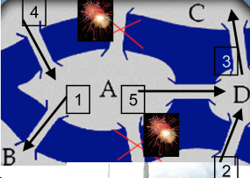
\includegraphics{images/ch1/konisberg_bridges_4.png}
\caption{images}
\end{figure}

Source: Wikipedia

    \hypertarget{research-questions-for-legal-network-analysis}{%
\subsection{1.3 Research Questions for Legal Network
Analysis}\label{research-questions-for-legal-network-analysis}}

Network analysis focuses on relational patterns and structures that
arise from interaction between the entities (called 'nodes). This
approach allows analyzing a variety of networks, ranging from online
cyber communities and corporate relations networks to social movements,
political affiliations, sports clubs, and scholarly communities.
Although there are many different categories of networks, they can more
generally be grouped under the headings of technological networks
(distribution, transportation, Internet), information networks
(citation, discourse), and social networks (friends, professional)
(Newman 2018).

Network analysis can also be a relevant approach in a legal context. We
refer to these situations as legal network analysis. Various studies
exist where it has been applied to examine citation patterns of courts
to identify sub-topics and precedents within the network. The network
analytical approach can also be relevant for other purposes, for
instance when conducting research on organized crime syndicates and how
they are organized.

Here, we illustrate the use of network analysis in the legal domain by
means of several examples. Because legal network analysis often concerns
the application to court decisions or legislation, this will be
reflected in the examples that are discussed.

\begin{itemize}
\item
  In \href{https://doi.org/10.1111/eulj.12077}{``\emph{Goodbye van Gend
  en Loos, Hello Bosman}?''} Derlen and Lindholm used network analysis
  to compare the precedent value of cases of the Court of Justice of the
  European Union. Using citation counts as a metric, the authors found
  that less well-known cases like \emph{Bosman} and \emph{Dassonville}
  garnered more citations than famous cases like \emph{van Gend and
  Loos}, \emph{Costa v. ENEL}, \emph{Brasserie du Pêcheur}, and
  \emph{United Brands}.
\item
  Fowler and Leon's
  \href{https://doi.org/10.1016/j.socnet.2007.05.001}{``\emph{The
  Authority of Supreme Court Precedent}''} is a seminal study of network
  analysis in the legal field. This study analyzed the complete network
  of 30,288 majority opinions written by the U.S. Supreme Court and the
  citations in the opinions from 1754 to 2002. The authors found that
  reversed judgments are more important than other judgments, that
  judgments that overrule previous judgments become and remain more
  important, and that overruling decisions are grounded in past
  precedents. To explore the citation patterns over time, the authors
  partitioned the network based on periods (e.g., 1754-1800, 1754-1801,
  1754-1802, etc.) and compared the citations for each of the
  partitions. This allowed the authors to, for instance, observe that
  some judgments would gather their citations in the first years after
  its publication whereas other judgments would continuously collect
  citations over time.
\item
  In \href{https://doi.org/10.1017/S0007123411000433}{``\emph{Precedent
  in International Courts: A Network Analysis of Case Citations by the
  European Court of Human Rights}''} Lupu and Voeten analyzed 7,319
  European Court of Human Rights (ECtHR) judgments up to and including
  2006. Among other things, the authors were interested in the question
  of whether the judgments could be grouped based on substantive reasons
  (as opposed to the judgments being grouped based on, for instance, the
  respondent country). The authors found that the different communities
  consisted of different topics. For instance, one community consisted
  of judgments with the keywords `life', `effective remedy', `positive
  obligation', and `inhuman treatment', whereas other communities
  concerned procedural matters (`fair hearing', `lawful arrest or
  detention', `reasonable time') or fundamental freedoms (`freedom of
  expression', `necessary in a democratic society', `protection of the
  rights of others', `respect for private life').
\item
  In \href{https://doi.org/10.1023/A:1004759418226}{``\emph{Spreading
  and Shifting Costs of Lateral Control Among Peers: A Structural
  Analysis at the Individual Level}}, Lazega and Krackhardt used network
  analysis in order to understand the complex dynamics taking palce
  within a firm. The authors studied a corporate law firm with 71
  lawyers (36 partners and 35 associates) in three offices. Their work
  provided perspectives on how partners foster cooperation, resolve
  conflicts, and preserve institutional stability. The study identified
  different leverage styles employed by partners, reflecting varying
  levels of seniority and approaches to managing control costs.
\item
  Network analysis can also be used for intelligence and criminal
  investigations. One may identify central members and their roles in
  the network or map interactions between entities in the network.
  Different entities may be connected, for instance, individuals and
  addresses, addresses and crime locations, individuals and
  organizations, individuals and individuals (through communication),
  and crimes and crime features. This way, certain types of crimes may
  be clustered and connected to certain individuals, organizations, or
  types of individuals and organizations. For an example of this type of
  research see Seidler and Adderley's
  \href{https://doi.org/10.1350/ijps.2013.15.4.321}{``\emph{Criminal
  Network Analysis inside Law Enforcement Agencies: A Data-Mining System
  Approach under the National Intelligence Model}''}.
\item
  Network analysis has also been used in patent studies, for instance,
  to test whether a certain inventor (e.g., Bill Gates) has invented in
  a wider variety of areas than another inventor (e.g., Mark
  Zuckerberg). This type of analysis can be carried out by computing the
  similarity score between inventions after having placed the inventor's
  creations within a semantic framework. The similarity scores can be
  used to construct an expertise network that visualizes the inventor's
  innovations along with their respective similarities. Such an analysis
  can yield insight into possible patent rights infringements. For an
  example of this approach see Whalen, Lungeanu, DeChurch and
  Contractor's work in
  \href{https://doi.org/10.1111/jels.12261}{``\emph{Patent Similarity
  Data and Innovation Metrics}''}.
\end{itemize}

Based on the examples above, we can already identify a variety of
possible research questions one may want to answer with legal network
analysis:

What are the most important precedents?

How does case importance change over time?

Have certain legal topics or legal concepts gained or lost importance
over time?

Which clusters of decisions can be distinguished?

How do law firm partners exercise control over others in the firm?

How can network analysis be used to provide relevant timely and
actionable intelligence for criminal networks?

These sample questions illustrate that legal network analysis can be
used for the empirical or computational studies of both positive law
(law as it exists in codes and decisions) and of social phenomena
relevant to the law (e.g., criminal networks, corporate influence).

In this book, we use a variety of examples to explain key concepts of
legal network analysis. We use a network on drone legislation throughout
the book to show how a network analysis is conducted and evolves from a
research question all the way to the software used to answer the
question. The drone example is derived from a study that explored
whether the finding of possible relevant drone legislation can be
automated through reference-based retrieval. It focused on whether the
references in legislation to other laws can help identify possibly
relevant drone legislation. The
\href{https://www.mdpi.com/2504-446X/7/8/490}{study} compared the
results to the laws identified by subject matter experts.

For the purpose of this book, we modify the study's research question
and ask which clusters of legislation can be distinghuished and which
laws are the most important in the network. In principle, almost all
legislation can become relevant, ranging from general liability law
(e.g., in instances of drone accidents) to environmental law (e.g.,
disturbing wildlife), yet it can nevertheless be interesting to focus on
specific clusters of laws related to drone regulation. For instance,
aviation law directly governs the use of drones in airspace while
privacy laws become relevant when drones are used for surveillance or
data collection. By analyzing how drone legislation is related to other
pieces of legislation we can better understand which laws are central to
a lawful use of drones in various sectors. We are hence interested in
whether citations from and to specific drone legislation help us
identify certain areas of the law (e.g., rules regarding drones'
technical requirements, rules regarding drone flights, privacy
legislation, cybersecurity) that might be relevant and which laws are
the most central ones in the network of drone legislation.

    


    
    
    
